This chapter presents the introduction to the software metrics as the important tool for evaluation of quality and productivity of the software development product. Also the classification of the software metrics, description the different measurements of software metrics in general and the most popular software metrics tools are included in this chapter.


\section{Definition of Software Metrics}

Software metrics are the attributes of the software systems that deals with the measurements of the software product and process by which it is developed~\cite{metrix}.
 
A software metric is a measure of characteristics of software which are countable or quantifiable. The importance of software metrics is valuable for many reasons, including planning work items, measuring software performance, measuring productivity, and many other uses.

Software developers must recognize the principles of software metrics that involve cost,schedule find quality goals, quantitative goals, comparison of plans with actual performance throughout development, monitoring data trends for indication of likely problems, metrics presentation, and investigation of data values.

There are some metrics within the process of software development, that are all related to each other. Metrics can be related to the four functions of management:

\begin{itemize}
	\item Controlling.
	\item Planning.
	\item Improving.
	\item Organising.
\end{itemize}

The aim of analyzing and tracking software metrics is to find out the quality of the particular product or process, enchance its quality and forecast the quality once the software development project is done. On a more detailed level, software development managers try to:

\begin{itemize}
	\item Manage workloads.
	\item Increase return on investment (ROI).
	\item Reduce overtime.
	\item Identify areas of improvement.
	\item Reduce costs.
\end{itemize}

These goals can be polished by providing information and clarity overall the organization about complex software development projects. Metrics are an essential value of quality assurance, performance, management, debugging, and estimating costs,a nd they are valuable for both development team leaders and developers:

\begin{itemize}
	\item Teams of software developers can use software metrics to interact between the status of
	software development projects, pinpoint and address issues, and observe, improve on,
	and manage their workflow better.
	\item Managers of software can use software metrics to track, identify, communicate and prioritize any
	issues to foster better team productivity. This permits effective management and allows
	prioritization and assessment of problems within software development projects. The
	sooner managers can find software problems, the easier and less-expensive the process of troubleshooting.
\end{itemize}

Software metrics provide an assessment of the impact of decisions made through the process of development of software projects. This helps managers prioritize and assess performance goals and objectives.

\section{Classification of software metrics}

Software metrics are broadly classified as product metrics and process metrics as shown in Figure \ref{fig:classification} ~\cite{metrics2}.
\begin{figure}[h]
	\centering
	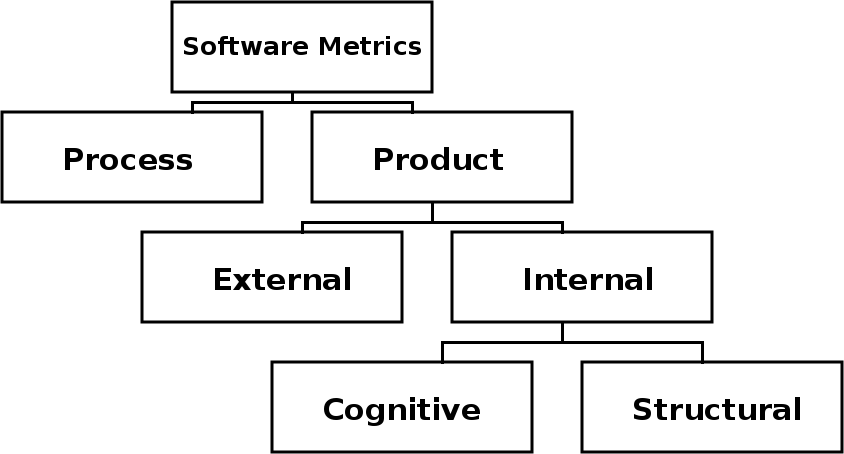
\includegraphics[height=55mm]{figures/classification.png}
	\caption{Classification of software metrics.}
	\label{fig:classification}
\end{figure}

Process metrics are numerical values that depict a software process such as the amount of time require to debug a module~\cite{metrics2}. They are measures of the software development process, such as: overall development time and type of methodology used. Process metrics are collected across all projects and over long periods of time. Their intent is to provide indicators that lead to longterm software process improvement.

Product metrics are measures of software project and are used to monitor and control the project. These metrics measures the complexity of the software design size of the final program number of pages of documentation produced. They enable a software project manager to:

\begin{itemize}
	\item[--] minimize the development time by making the adjustments necessary to avoid delays
	and potential problems and risks.
	\item[--] assess product quality on an ongoing basis and modify the technical approach to improve
	quality.
\end{itemize}

Product metrics are measures of the software product of any stage of its development,from requirements to installed system. Product metrics may measure: the complexity of the software design, the size of the final program, the number of pages of documentation prodused.
Product metrics can be internal or external. External attributes of an entity can be measured only with respect to how the entity relates with the environment and therefore can be measured only indirectly. For example, reliability, an external attribute of a program, does not depend only on the program itself but also on the compiler, machine and user. Productivity, an external attribute of a person, clearly depends on many factors such as the kind of process and the quality of the software delivered. Internal product metrics can be measured only based on the entity and therefore the measures are direct. For example, size is an internal attribute of any software document.

Internal product metrics are subdivided in two categories: cognitive
complexity metrics and structural complexity metrics. Cognitive complexity metrics measure the effort required by developers to understand a system. They aim at discovering the cause of the complexity, which requires understanding human mental processes and details of the software system under development. Structural complexity metrics use the interactions within and among modules to measure a system’s complexity. One of the oldest and most commonly used structural complexity metrics is the number of source lines of code.

Another classification of software metrics is as follows:

\begin{enumerate}
	\item Objective metrics.
	\item Subjective metrics
\end{enumerate}

Objective metrics always results in identical values for a given metric as measured by two or more qualified observers. Whereas subjective metrics are those that even qualified observers may measure different values for a given metric since their subjective judgment is involved in arriving at the measured value.
%%____________________________________________________________________________

\section{Types Of Software Metrics}

It is now apparent that software metrics are important in software
engineering. Symons stated that "a reliable and credible method
for measuring the software development cycle is needed that has a reasonable
theoretica1 basis and that produces results that practitioners can trus" Hence,software metrics have been used to measure a wide range of software
engineering activities.

\subsection{Size-Oriented metrics}

Size-oriented metrics are used to analyze the quality of software.

\textbf{Lines of Code (LOC)}

Lines Of Code (also known as Source Lines of Code - SLOC) is a metric generally used to
evaluate a software program or codebase according to its size. It shows how many lines of source
code there is in the application, namespace, class or method. LoC can be used to: check the size
of code units and estimate the size of project. LOC is the popular and simplest one.
There are two major types of SLOC measures: 

\begin{description}
	\item[Physical SLOC (LOC)] Physical SLOC is a count of lines in the text of the program's source code including comment.
	\item[Logical SLOC(LLOC)] Logical LOC tries to count the number of "statements", but their specific definitions are tied to specific computer languages.
\end{description}

Physical SLOC measures are sensitive to logically irrelevant formatting and style conventions, while logical LOC is less sensitive to formatting and style conventions. Unfortunately, SLOC measures are often stated without giving their definition, and logical LOC can often be significantly different from physical SLOC.

\subsection{Object Oriented metrics (OO)}

Chidamber and Kemerer have specified a several metrics for object oriented
designs. All of these metrics are referred to the separate class but not to the whole system.

\textbf{Number Of Methods (NOM)}

The Number Of Methods metric is used to calculate the average count of all class operations per class. A class must have some, but not an excessive number of operations.This information is useful when identifying a lack of primitiveness in class operations (inhibiting
re-use), and in classes which are little more than data types.

\textbf{Number Of Children (NOC)}

NOC is a number of immediate subclasses subordinated to a class in the class hierarchy. NOC counts the number of subclasses belonging to a class.

NOC measures the breadth of a class hierarchy, where maximum DIT measures the depth. Depth is generally better than breadth, since it promotes reuse of methods through inheritance. NOC and DIT are closely related. Inheritance levels can be added to increase the depth and reduce the breadth.

A high NOC, a large number of child classes, can indicate several things: 
\begin{itemize}
	\item High reuse of base class. Inheritance is a form of reuse.
	\item Base class may require more testing.
	\item Improper abstraction of the parent class. 
	\item Misuse of sub-classing. In such a case, it may be necessary to group related classes and introduce another level of inheritance.
\end{itemize}

A class with a high NOC and a high WMC indicates complexity at the top of the class hierarchy. The class is potentially influencing a large number of descendant classes. This can be a sign of poor design. A redesign may be required.

Not all classes should have the same number of sub-classes. Classes higher up in the hierarchy should have more sub-classes then those lower down.


\textbf{Weighted Methods per Class (WMC)}

This metric is the sum of complexities of methods defined in a class. It therefore represents the
complexity of a class as a whole and this measure can be used to indicate the development and
maintenance effort for the class. Classes with a large Weighted Methods Per Class value can often be refactored into two or more classes.

\textbf{Coupling Between Object classes (CBO)}

CBO classes metric demonstrates the number of classes coupled to a given class. This coupling can happen throuhg:
\begin{itemize}
	\item Properties or parameters. 
	\item Method call. 
	\item Method arguments or return types.
	\item Class extends.
	\item Variables in methods
\end{itemize}

Coupling among classes is needed for a system to do useful work, but redundant coupling makes the system more difficult to reuse and maintain. At project or package level, this metric shows the average number of classes used per class.

\textbf{Depth of Inheritance Tree (DIT)}

Depth of Inheritance Tree (DIT) is the maximum length of a path from a class to a root class in the inheritance structure of a system. DIT measures how many super-classes can affect a class. DIT is only applicable to object-oriented systems.

The deeper a class is in the hierarchy, the more methods and variables it is likely to inherit, making it more complex. Deep trees as such indicate greater design complexity. Inheritance is a tool to manage complexity, really, not to not increase it. As a positive factor, deep trees promote reuse because of method inheritance.

C\&K suggested the following consequences based on the depth of inheritance:
\begin{itemize}
	\item Deeper trees establish greater design complexity, since more classes and methods are involved
	\item The deeper a class is in the hierarchy, the greater the number of methods it is going to inherit, making it more complex to foresee its behavior
	\item The deeper a particular class is in the hierarchy, the greater the possible reuse of inherited methods 
\end{itemize}

\textbf{Response For a Class (RFC)} 
The Response for Class (RFC) metric is the total number of methods that can potentially be executed in response to a message received by an object of a class. This number is the sum of the methods of the class, and all distinct methods are invoked directly within the class methods. Additionally, inherited
methods are counted, but overridden methods are not, because only one method of a particular signature will always be available to an object of a given class.

A large RFC has been found to indicate more faults. Classes with a high RFC are more complex and harder to understand. Testing and debugging is complicated. A worst case value for possible responses will assist in appropriate allocation of testing time.
%%___________________________________________________
\subsection{Complexity metrics}
Complexity is an important aspect for software quality assessment and must be appropriately addressed in service-oriented architecture\cite{complexity}. One  of  the  key  aims  of  complexity  metrics  is  to  predict modules   that are fault-prone post-release~\cite{complexity2}. This metrics are one of the most difficult software metrics for understanding.

\textbf{McCabe's Cyclomatic Complexity (MVG)}

McCabe's cyclomatic complexity is a software quality metric that shows the complexity of a software program. Complexity is inferred by summarizing the number of linearly independent paths through the program. The higher the number the more complex the code.

A pragmatic approximation to this can be found by counting language keywords and operators which introduce extra decision outcomes.
%%_______________________________
\subsection{Structural Metrics}

\textbf{Fan-In and Fan-Out metrics (FIN and FOUT)}

It's a structural metrics which measures inter-module complexities. 
\begin{description}
	\item[Fan-out] Is the number of modules that are called by a given module.
	\item[Fan-in] Is the number of modules that call a given module.
\end{description}

Fan-out and fan-in metrics reflect structure dependency~\cite{fanin}.
This structural metrics were first defined by Henry.
This metrics can be applied both at module level and function level. This metrics just puts a number on how complex is interlinking of different modules or functions. Unlike Cyclomatic complexity you cannot put a number and say it cannot go beyond this number. This is used just to size up how
difficult it will be to replace a function or module in your application and how changes to a function or module can impact other functions or modules. Sometimes you can put restriction on number of Fan-Out a function has to avoid cluttering your function but is not a widely accepted practice.

%%______________________________________________________

\subsection{Cohesion metrics}
Cohesion is an important software quality attribute and high cohesion is one of characteristics of well-structured software design~\cite{cohesion}.
Cohesion metrics analyze the connection between methods of a class.
Module cohesion indicates relatedness in the functionality of a software module~\cite{cohesion2}.

\textbf{Lack of Cohesion in Methods (LCOM)}

LCOM calculates the number of cohesiveness present, how well a system was designed and how complex a class is. LCOM is a count of the number of method pairs whose similarity is zero,minus the count of method pairs whose similarity is not zero. LCOM is probably the most controversial and argued over of the C\&K metrics.

C\&K's rationale for the LCOM method was as follows:
\begin{itemize}
	\item Lack of cohesion implies classes should probably be split into two or more subclasses.
	\item Cohesiveness of methods within a class is desirable, since it promotes encapsulation.
	\item Low cohesion increases complexity, thereby increasing the likelihood of errors during the development process.
	\item Any measure of disparateness of methods helps identify flaws in the design of classes. 
\end{itemize}

Although there is a fair amount of debate about how to calculate LCOM and it features in a lot of metrics sets an increasing number of researchers suggest that it is not a particularly useful metric. Perhaps this is also reflected in there being a fair amount of debate about how to calculate LCOM but very little on how to interpret it and how it fits in with other metrics. 

\textbf{Tight and Loose Class Cohesion (TCC and LCC)}

TCC(Tight Class Cohesion) and LCC(Loose Class Cohesion) metrics measure  the  relative number of directly-connected pairs of methods and the   relative   number of directly- or indirectly- connected pairs of methods.
The Tight Class Cohesion metric measures the cohesion between the public methods of a class. That is the relative number of directly connected public methods in the class. Classes having a low cohesion indicate errors in the design.

TCC considers two methods to be connected if they share the  use  of  at  least  one  attribute.  A  method  uses  an  attribute if the attribute appears in the method’s body or  the  method  invokes  directly  or  indirectly  another method   that   has   the   attribute   in   its   body.   
The higher TCC and LCC, the more cohesive and thus better the class.

In this Section we focused our attention on all posible software metrics. In the next Chapter we will define metrics which are used to describe various aspects of Erlang projects. 
%%______________________________________________________________________

\section{Software Metric Tools}
There are a lot of software metrics have been developed and numerous tools exist to gather the metrics from program representations. This large number of tools allows a user to choose the tool best suited as per the use requirements for example it's handling, tool support, cost etc. This is accepted that the metrics computed by the metric tools are same for all the metric tools. One can think of a software metric tool as a program which implements a set of software metrics definitions. It allows to access a software system according to the metrics by extracting the required entities from the software ad providing the corresponding metric values. There are
some criteria for selecting the proper metric tools as the availability of the software tools can make confusion. One such criterion is that the tools must have to calculate any form of software metrics. Majority metric tools are available for Java programs. Many tools are just code counting
tool, they basically count the variants of the lines of code(LOC) metric. The specific criteria areas follows language: Java(source or byte code), metrics: well known object oriented metrics on class level, license: freely available.

\subsection{CCCC}

It is a little command-line tool that generates metrics from the source code of a C or C++ project. The output of the tool is a simple HTML website with information about all your sources. It generates reports on various metrics including lines of code (LOC) and metrics proposed by Chidamber\&Kemererand Henry\&Kafura. CCCC has been developed as freeware, and is released in source code form. Users are encouraged to compile the program themselves, and to modify the source to reflect their preferences and interests.

CCCC will process each of the files specified on the command line (using standard wildcard processing were appropriate. For each file, named, CCCC will examine the extension of the filename, and if the extension is recognized as indicating a supported language, the appropriate parser will run on the file. As each file is parsed, recognition of certain constructs will cause records to be written into an internal database. When all files have been processed, a report on the contents of the internal database
will be generated in HTML format. By default the main summary HTML report is generated to the file cccc.htm in a subdirectory called .cccc of the the current working directory, with detailed reports on each module (i.e. C++ or Java class) identified by the analysis run).

In addition to the summary and detailed HTML reports, the run will cause generation of corresponding summary and detailed reports in XML format, and a further file called cccc.db to be created. cccc.db will contain a dump of the internal database of the program in a format delimited with the character '@' (chosen because it is one of the few characters which cannot legally appear in C/C++ non -comment source code).

The report contains a number of tables identifying the modules in the files submitted and covering:
\begin{enumerate}
	\item Measures of the number and type of the relationships each module is a party to either as a client or a supplier.
	\item Measures of the procedural volume and complexity of each module and its functions;. 
	\item A summary report over the whole body of code processed of the measures identified above.
	\item Identification of any parts of the source code submitted which the program failed to parse.
\end{enumerate}

This tool can measure the following metrics:
\begin{itemize}
	\item Fan-In Fan-Out()FIN and FOUT).
	\item Lines of Code (LOC). 
	\item Numbe r Of Children(NOC).
	\item Weighted Methods per Class(WMC).
	\item McCabe's Cyclomatic Complexity(MVG).
	\item Number Of Methods (NOM).
\end{itemize}

\subsection{Chidamber\&Kemerer}

The program counts Chidamber and Kemerer object-oriented metrics by introspection the bytecode of compiled Java files.It is open source command line tool. The program counts the following six metrics for each class, and displays them on its standard output, following the class's name.

This tool can measure the following metrics:

\begin{itemize}
	\item Depth of Inheritance Tree (DIT).
	\item Weighted Methods per Class(WMC).
	\item Numbe r Of Children(NOC).
	\item Coupling Between Object classes (CBO).
	\item Lack of Cohesion in Methods (LCOM).
	\item Response For a Class (RFC).
\end{itemize}

\subsection{Analyst4j}
It is built on the Eclipse platform and can be downloaded as a standalone Rich Client Application or also as an Eclipse
IDE plugin. Its features are search, metrics analyzing, quality analyzing, report generating for Java programming.
Analyst4j software are most popular to find out the quality related metrics. This tool is based on Chidamber\&Kemerer metrics.

This tool can measure the following metrics:
\begin{itemize}
	\item Weighted Methods per Class(WMC).
	\item Lines of Code (LOC). 
	\item Coupling Between Object classes (CBO).
	\item Depth of Inheritance Tree (DIT).
	\item Response For a Class (RFC).
	\item Number Of Children(NOC).
	\item Lack of Cohesion in Methods (LCOM).
	\item Number Of Methods (NOM).
\end{itemize}

\subsection{OOMeter}

OOMeter is a software metric tool for measuring the quality attributes of Java and C\# source code and UML models, stored in XMI format. OOMeter has a rich collection of object-oriented software metrics. This is the Eclipse plugin. It provides an querying language for object-oriented code similiar to SQL which
allows to search for measure code metrics, bugs etc.

OOMeter provides an interface for users to define custom metrics through java classes that implement a certain interface. It supports export of metric results to a number of formats, including XML, HTML, delimited text, Microsoft Excel, etc.

This tool can measure the following metrics:

\begin{itemize}
	\item Weighted Methods per Class(WMC).
	\item Lines of Code (LOC). 
	\item Coupling Between Object classes (CBO).
	\item Depth of Inheritance Tree (DIT).
	\item Response For a Class (RFC).
	\item Numbe r Of Children(NOC).
	\item Tight Class Cohesion (TCC).
	\item Lack of Cohesion in Methods (LCOM).
\end{itemize}



\subsection{Eclipse Metrics plugin 1.3.6}

This is an open source dependency analyzer and metrics calculation plugin for Eclipse IDE. The plugin is also provided 
integrated  as  an  EasyEclipse  package.  The  plugin computes   the  various metrics and displays it in the integrated view.


This tool can measure the following metrics:

\begin{itemize}
	\item Weighted Methods per Class(WMC).
	\item Lines of Code (LOC). 
	\item Numbe r Of Children(NOC).
	\item Depth of Inheritance Tree (DIT).
    \item Number Of Methods (NOM).
\end{itemize}

\subsection{Eclipse Metrics plugin 3.4}
The  eclipse  plugin  3.4 developed  by  Lance  Walton  is  also  integrated  with Eclipse   and   is   available   for   all   Java   projects 
developed using the ID.E It is a open source tool. It counts various metrics in the moment of build cycles and shows warnings via the problem view of metrics range violations.

This tool can measure the following metrics:
\begin{itemize}
	\item Weighted Methods per Class(WMC).
	\item Lines of Code (LOC). 
	\item Lack of Cohesion in Methods (LCOM).
	\item Depth of Inheritance Tree (DIT).
\end{itemize}

\subsection{Semmle}

Semmle is the platform for analyzing that produces detailed report of the code base for one or more software projects. For every project that it analyzes, it calculates artifacts against rules that check for good practice. Analysis can be scheduled to run on a regular basis. The copy of the source code is checked out from the repository for analysis as part of this process. The code, and related artifacts, is checked against rules, defined using queries, to identify any alerts. Finally, metrics are calculated and data can be imported from third-party systems used by your company. A database is created, containing detailed information about the artifacts and every alert.

This tool can measure the following metrics:
\begin{itemize}
	\item Lack of Cohesion in Methods (LCOM).
	\item Depth of Inheritance Tree (DIT).
	\item Number Of Methods (NOM).
	\item Numbe r Of Children(NOC).
	\item Response For a Class (RFC).
\end{itemize}

\section{Measuring functional languages}
In previous section has been described sofrware metrics for object-oriented languages. However software metrics developed for imperative and object-oriented languages can also be used for measuring in functional programming languages like Erlang and Haskell. We can use the same metrics because several constructs as a class,  a module and a library are similar. All of this structures can be consider like collections of functions. If the chosen metric does not take the distinctive properties of these constructs into account (variables, method overrides, dynamic binding, visibility etc.), then it can be applied to these apparently diverse constructs ~\cite{metrics3}.

Dissimilarity between functional and imperative languages are in such features as difference in the level of nesting of blocks and control
structures, in several ways of connecting certain functions (for example, data flow and call graph), inheritance insted of cohesion and and simple cardinality metrics(lines of code, char of code).


Another difference functional programming languages from imperative languages is there are some constructs and properties that can be used only in functional programming languages as: list comprehensions, pattern matching, referential transparency of pure functions, currying, laziness of expression evaluation.

While these features raise the expressive power of functional languages,
most of the existing complexity metrics require some changes before they be-
come applicable to functional languages ~\cite{metrics3}.

There are general metrics are acceptable for functional languages:
\begin{itemize}
	\item \textbf{Branches of recursion}.This metric allows to measure how many times did the function call itself
	\item \textbf{Fun expressions and message passing constructs}.
	\item \textbf{Return points of a function}.
	\item There is possible to calculate metrics on a single clause of a function.
	\item There is possible to calculate metrics on a single clause of a function.
	\item \textbf{Otp used}. This metric allows measure OTP behaviours.
\end{itemize}

In the next chapter will be described all developed metrics for Erlang in details.



